% Options for packages loaded elsewhere
\PassOptionsToPackage{unicode}{hyperref}
\PassOptionsToPackage{hyphens}{url}
%
\documentclass[
]{article}
\usepackage{lmodern}
\usepackage{amssymb,amsmath}
\usepackage{ifxetex,ifluatex}
\ifnum 0\ifxetex 1\fi\ifluatex 1\fi=0 % if pdftex
  \usepackage[T1]{fontenc}
  \usepackage[utf8]{inputenc}
  \usepackage{textcomp} % provide euro and other symbols
\else % if luatex or xetex
  \usepackage{unicode-math}
  \defaultfontfeatures{Scale=MatchLowercase}
  \defaultfontfeatures[\rmfamily]{Ligatures=TeX,Scale=1}
\fi
% Use upquote if available, for straight quotes in verbatim environments
\IfFileExists{upquote.sty}{\usepackage{upquote}}{}
\IfFileExists{microtype.sty}{% use microtype if available
  \usepackage[]{microtype}
  \UseMicrotypeSet[protrusion]{basicmath} % disable protrusion for tt fonts
}{}
\makeatletter
\@ifundefined{KOMAClassName}{% if non-KOMA class
  \IfFileExists{parskip.sty}{%
    \usepackage{parskip}
  }{% else
    \setlength{\parindent}{0pt}
    \setlength{\parskip}{6pt plus 2pt minus 1pt}}
}{% if KOMA class
  \KOMAoptions{parskip=half}}
\makeatother
\usepackage{xcolor}
\IfFileExists{xurl.sty}{\usepackage{xurl}}{} % add URL line breaks if available
\IfFileExists{bookmark.sty}{\usepackage{bookmark}}{\usepackage{hyperref}}
\hypersetup{
  pdftitle={R Markdown},
  pdfauthor={Applied Machine Learning in Economics},
  hidelinks,
  pdfcreator={LaTeX via pandoc}}
\urlstyle{same} % disable monospaced font for URLs
\usepackage[margin=1in]{geometry}
\usepackage{color}
\usepackage{fancyvrb}
\newcommand{\VerbBar}{|}
\newcommand{\VERB}{\Verb[commandchars=\\\{\}]}
\DefineVerbatimEnvironment{Highlighting}{Verbatim}{commandchars=\\\{\}}
% Add ',fontsize=\small' for more characters per line
\usepackage{framed}
\definecolor{shadecolor}{RGB}{248,248,248}
\newenvironment{Shaded}{\begin{snugshade}}{\end{snugshade}}
\newcommand{\AlertTok}[1]{\textcolor[rgb]{0.94,0.16,0.16}{#1}}
\newcommand{\AnnotationTok}[1]{\textcolor[rgb]{0.56,0.35,0.01}{\textbf{\textit{#1}}}}
\newcommand{\AttributeTok}[1]{\textcolor[rgb]{0.77,0.63,0.00}{#1}}
\newcommand{\BaseNTok}[1]{\textcolor[rgb]{0.00,0.00,0.81}{#1}}
\newcommand{\BuiltInTok}[1]{#1}
\newcommand{\CharTok}[1]{\textcolor[rgb]{0.31,0.60,0.02}{#1}}
\newcommand{\CommentTok}[1]{\textcolor[rgb]{0.56,0.35,0.01}{\textit{#1}}}
\newcommand{\CommentVarTok}[1]{\textcolor[rgb]{0.56,0.35,0.01}{\textbf{\textit{#1}}}}
\newcommand{\ConstantTok}[1]{\textcolor[rgb]{0.00,0.00,0.00}{#1}}
\newcommand{\ControlFlowTok}[1]{\textcolor[rgb]{0.13,0.29,0.53}{\textbf{#1}}}
\newcommand{\DataTypeTok}[1]{\textcolor[rgb]{0.13,0.29,0.53}{#1}}
\newcommand{\DecValTok}[1]{\textcolor[rgb]{0.00,0.00,0.81}{#1}}
\newcommand{\DocumentationTok}[1]{\textcolor[rgb]{0.56,0.35,0.01}{\textbf{\textit{#1}}}}
\newcommand{\ErrorTok}[1]{\textcolor[rgb]{0.64,0.00,0.00}{\textbf{#1}}}
\newcommand{\ExtensionTok}[1]{#1}
\newcommand{\FloatTok}[1]{\textcolor[rgb]{0.00,0.00,0.81}{#1}}
\newcommand{\FunctionTok}[1]{\textcolor[rgb]{0.00,0.00,0.00}{#1}}
\newcommand{\ImportTok}[1]{#1}
\newcommand{\InformationTok}[1]{\textcolor[rgb]{0.56,0.35,0.01}{\textbf{\textit{#1}}}}
\newcommand{\KeywordTok}[1]{\textcolor[rgb]{0.13,0.29,0.53}{\textbf{#1}}}
\newcommand{\NormalTok}[1]{#1}
\newcommand{\OperatorTok}[1]{\textcolor[rgb]{0.81,0.36,0.00}{\textbf{#1}}}
\newcommand{\OtherTok}[1]{\textcolor[rgb]{0.56,0.35,0.01}{#1}}
\newcommand{\PreprocessorTok}[1]{\textcolor[rgb]{0.56,0.35,0.01}{\textit{#1}}}
\newcommand{\RegionMarkerTok}[1]{#1}
\newcommand{\SpecialCharTok}[1]{\textcolor[rgb]{0.00,0.00,0.00}{#1}}
\newcommand{\SpecialStringTok}[1]{\textcolor[rgb]{0.31,0.60,0.02}{#1}}
\newcommand{\StringTok}[1]{\textcolor[rgb]{0.31,0.60,0.02}{#1}}
\newcommand{\VariableTok}[1]{\textcolor[rgb]{0.00,0.00,0.00}{#1}}
\newcommand{\VerbatimStringTok}[1]{\textcolor[rgb]{0.31,0.60,0.02}{#1}}
\newcommand{\WarningTok}[1]{\textcolor[rgb]{0.56,0.35,0.01}{\textbf{\textit{#1}}}}
\usepackage{graphicx,grffile}
\makeatletter
\def\maxwidth{\ifdim\Gin@nat@width>\linewidth\linewidth\else\Gin@nat@width\fi}
\def\maxheight{\ifdim\Gin@nat@height>\textheight\textheight\else\Gin@nat@height\fi}
\makeatother
% Scale images if necessary, so that they will not overflow the page
% margins by default, and it is still possible to overwrite the defaults
% using explicit options in \includegraphics[width, height, ...]{}
\setkeys{Gin}{width=\maxwidth,height=\maxheight,keepaspectratio}
% Set default figure placement to htbp
\makeatletter
\def\fps@figure{htbp}
\makeatother
\setlength{\emergencystretch}{3em} % prevent overfull lines
\providecommand{\tightlist}{%
  \setlength{\itemsep}{0pt}\setlength{\parskip}{0pt}}
\setcounter{secnumdepth}{5}

\title{R Markdown}
\author{Applied Machine Learning in Economics}
\date{}

\begin{document}
\maketitle

{
\setcounter{tocdepth}{2}
\tableofcontents
}
Open a new markdown:

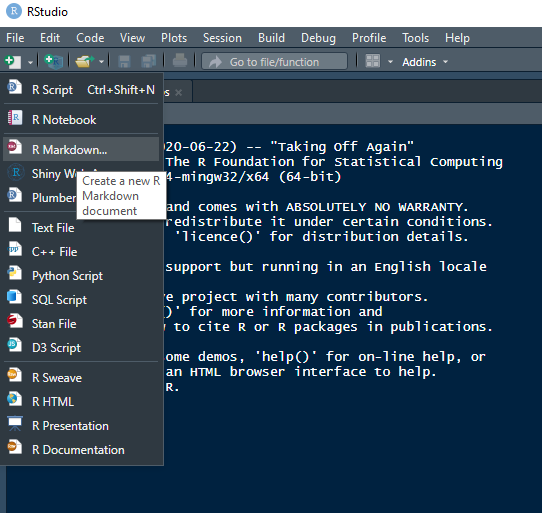
\includegraphics{new markdown.png}

Explore around what types of markdowns you can make. Then select an html
document. Knit this document by typing \texttt{Ctrl-Shift-k}

Now you may follow this document

\hypertarget{section-1}{%
\section{Section 1}\label{section-1}}

\begin{center}\rule{0.5\linewidth}{0.5pt}\end{center}

\hypertarget{this-will-one.one}{%
\subsection{This will one.one}\label{this-will-one.one}}

\hypertarget{not-1.1.2}{%
\subsubsection{not 1.1.2}\label{not-1.1.2}}

\hypertarget{not-in-table-of-contents}{%
\paragraph{Not in table of contents}\label{not-in-table-of-contents}}

\hypertarget{rmarkdown-basics}{%
\section{RMarkdown Basics}\label{rmarkdown-basics}}

\begin{center}\rule{0.5\linewidth}{0.5pt}\end{center}

Here are some fundamentals to writting in RMarkdown.

\hypertarget{writing-text}{%
\subsection{Writing text}\label{writing-text}}

\begin{center}\rule{0.5\linewidth}{0.5pt}\end{center}

This is how to write text in RMarkdwon. Notice writing on the next line
stays in the same paragraph.

This is how you start a new paragraph. Wrap you words in * to get
\emph{italics}. Using two *s will produce \textbf{bolface}. There are
other things that we can do too, like making lists.

\begin{enumerate}
\def\labelenumi{\arabic{enumi}.}
\tightlist
\item
  Item 1
\item
  Item 2

  \begin{enumerate}
  \def\labelenumii{\alph{enumii}.}
  \setcounter{enumii}{1}
  \tightlist
  \item
    Notice how we had to align in the RMarkdown code

    \begin{itemize}
    \tightlist
    \item
      You can choose whether you use numers. or letters. but RMarkdown
      chooses the symbols for you :(
    \end{itemize}
  \end{enumerate}
\end{enumerate}

This is how we reference inline code like \texttt{R}'s base function
\texttt{plot} is as pretty as \texttt{ggplot2}'s function
\texttt{ggplot}.

To write math, we can use some limited \texttt{latex} features. Like if
we wanted to show a regression formula inline:
\(y_i = \alpha + x_i\beta + \epsilon_i\). Alternatively, if we have
important math like the geometric series identity, we can make it stand
out: \[
2^2 = 4\\
\begin{align*}
  \sum_{n=0}^\infty ar^n & = a \left( \frac{1}{1-r} \right)\\
  & = \frac{a}{1-r}\\
  & \text{for } |r| < 1
\end{align*}
\]

If we want to link sections, we do this
\protect\hyperlink{section-1}{Section 1}. Or if we need to link a
website, we do this while making sure to include https. A really useful
\href{https:/www.bookdown.org/yihui/rmarkdown}{resource} for additional
RMarkdown tips and tricks.

This is how we include images in our markdown.
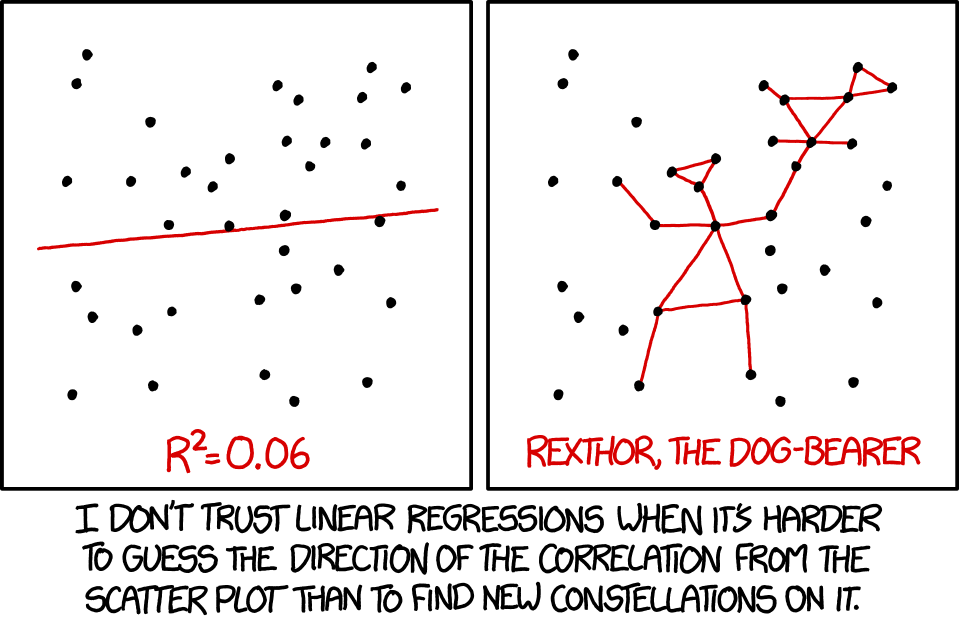
\includegraphics{linear_regression_2x.png}

\hypertarget{writing-code}{%
\subsection{Writing Code}\label{writing-code}}

Here is the basic to writing code chunks.

\begin{Shaded}
\begin{Highlighting}[]
\KeywordTok{print}\NormalTok{(}\StringTok{'hello world'}\NormalTok{)}
\end{Highlighting}
\end{Shaded}

\begin{verbatim}
## [1] "hello world"
\end{verbatim}

\#@@@@ RUN INSIDE SCRIPT

The first part of the curly braces tells you what language you are using
and the name of the chunk. Then options can be set up using commas after
the chunk name by setting them to \texttt{TRUE} or \texttt{FALSE}. Some
major options all of which have default of \texttt{TRUE} are:

\begin{itemize}
\tightlist
\item
  \texttt{include} - Whether or not to be included in the document
\item
  \texttt{echo} - Displays the code
\item
  \texttt{results} - Displays the output of the code
\item
  \texttt{messages} - Display messages from the functions if they have
  them.
\end{itemize}

\#@@@@ \#@@@@ \#@@@@ \#@@@@ Some general advice. Copy and paste into
word. Typos, not a native language, or if you are native but sometimes
english is really hard. \#@@@@ \#@@@@ \#@@@@

\hypertarget{an-example-assignment}{%
\section{An example assignment}\label{an-example-assignment}}

\begin{center}\rule{0.5\linewidth}{0.5pt}\end{center}

We must do the following:

\begin{enumerate}
\def\labelenumi{\arabic{enumi}.}
\tightlist
\item
  load ggplot2
\item
  load in gapminder\_2007
\item
  produce a correlation matrix
\item
  obtain mean and standard deviation of the America's GDPc
\item
  Summary stats of life expectancy for countries with GDPC less than
  \$10,000
\item
  Replicate plot from last lecture
\end{enumerate}

\hypertarget{load-in-ggplot2-and-gapminder_2007}{%
\subsection{Load in ggplot2 and
gapminder\_2007}\label{load-in-ggplot2-and-gapminder_2007}}

\begin{center}\rule{0.5\linewidth}{0.5pt}\end{center}

Done, but I am not going to show you!

\hypertarget{produce-three-sets-of-statistics}{%
\subsection{Produce Three Sets of
Statistics}\label{produce-three-sets-of-statistics}}

\begin{center}\rule{0.5\linewidth}{0.5pt}\end{center}

Here is a correlation matrix GDP per capita, life expectancy, and
population.

\begin{verbatim}
##            gdpPercap    lifeExp         pop
## gdpPercap  1.0000000 0.67866240 -0.05567560
## lifeExp    0.6786624 1.00000000  0.04755312
## pop       -0.0556756 0.04755312  1.00000000
\end{verbatim}

Here is the mean and standard deviation of the America's GDP per capita.

\begin{Shaded}
\begin{Highlighting}[]
\NormalTok{americas =}\StringTok{ }\NormalTok{gm[gm}\OperatorTok{$}\NormalTok{continent }\OperatorTok{==}\StringTok{ 'Americas'}\NormalTok{, ]}
\NormalTok{m =}\StringTok{ }\KeywordTok{mean}\NormalTok{(americas}\OperatorTok{$}\NormalTok{gdpPercap)}
\NormalTok{m =}\StringTok{ }\KeywordTok{round}\NormalTok{(m, }\DecValTok{2}\NormalTok{)}
\NormalTok{s =}\StringTok{ }\KeywordTok{round}\NormalTok{(}\KeywordTok{sd}\NormalTok{(gm[gm}\OperatorTok{$}\NormalTok{continent }\OperatorTok{==}\StringTok{ 'Americas'}\NormalTok{, }\StringTok{'gdpPercap'}\NormalTok{]), }\DecValTok{2}\NormalTok{)}
\KeywordTok{print}\NormalTok{(}\KeywordTok{paste0}\NormalTok{(}\StringTok{"Americas' mean: "}\NormalTok{, m))}
\end{Highlighting}
\end{Shaded}

\begin{verbatim}
## [1] "Americas' mean: 11003.03"
\end{verbatim}

\begin{Shaded}
\begin{Highlighting}[]
\KeywordTok{print}\NormalTok{(}\KeywordTok{paste}\NormalTok{(}\StringTok{"Americas' standrad deviation:"}\NormalTok{, s))}
\end{Highlighting}
\end{Shaded}

\begin{verbatim}
## [1] "Americas' standrad deviation: 9713.21"
\end{verbatim}

And finally here are the summary statistics of life expectancy for
countries with less than \$10,000 gdp per capita

\begin{Shaded}
\begin{Highlighting}[]
\KeywordTok{summary}\NormalTok{(gm[gm}\OperatorTok{$}\NormalTok{gdpPercap }\OperatorTok{<}\StringTok{ }\DecValTok{10000}\NormalTok{, }\StringTok{'lifeExp'}\NormalTok{])}
\end{Highlighting}
\end{Shaded}

\begin{verbatim}
##    Min. 1st Qu.  Median    Mean 3rd Qu.    Max. 
##   39.61   52.11   62.88   61.37   71.97   78.78
\end{verbatim}

\hypertarget{replicate-last-lectures-plot}{%
\subsection{Replicate Last Lectures
Plot}\label{replicate-last-lectures-plot}}

\begin{center}\rule{0.5\linewidth}{0.5pt}\end{center}

Here is the plot we already made.

\includegraphics{R-Markdown_files/figure-latex/eda-1.pdf}

\end{document}
